We begin by considering the phenomenon of increasing efficiency in repeated reference games: speakers use detailed descriptions at the outset but converge to an increasingly compressed shorthand while remaining understandable to their partner.
While this phenomenon has been extensively documented, to the point of serving as a proxy for measuring common ground, it has continued to pose a challenge for models of communication.
 \begin{figure*}
	\centering
    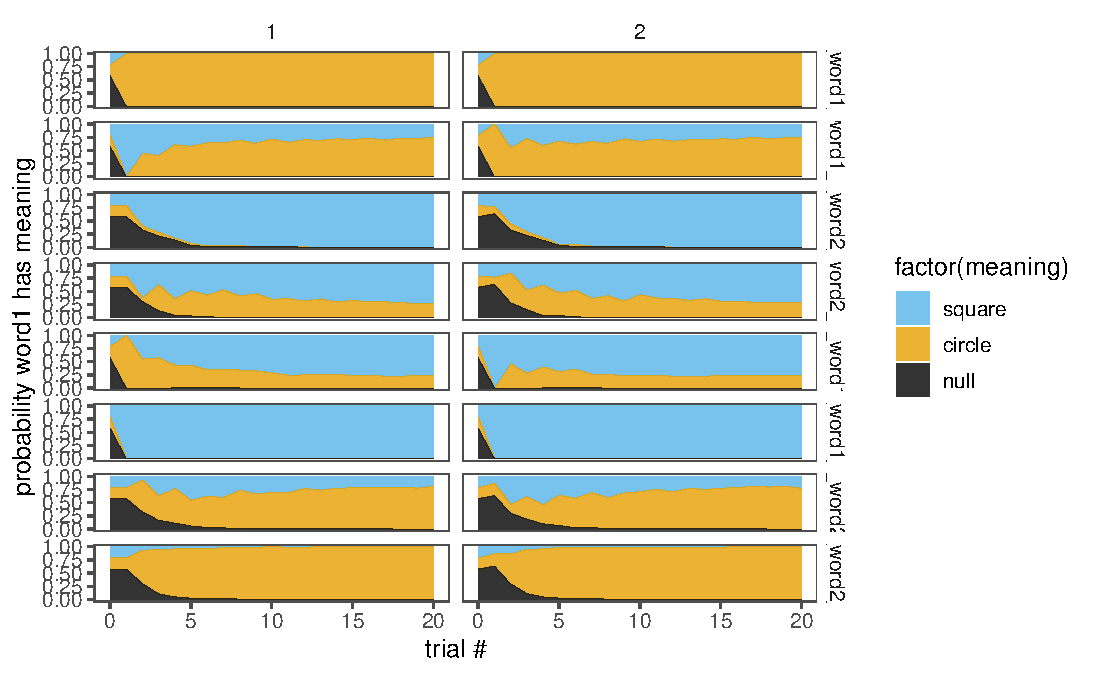
\includegraphics[scale=.6]{sec1-arbitrariness}
    \caption{\emph{Path-dependence of conventions.} The average trajectory of each agent's beliefs about the meaning of $u_1$, $\phi(u_1)$, is shown in blue and orange following all eight possible outcomes of the first trial in Simulation 1.1. For each of the two possible targets, the speaker could choose to produce either of the two utterances, and the listener could respond by choosing either of the two objects. In the cases where the listener chose correctly (marked with a checkmark), agents subsequently conditioned on the same data and rapidly converged on a system of meaning consistent with this feedback. For example, in the first row, when $u_1$ was successfully used to refer to the circle, both agents subsequently believe that $u_1$ means \emph{circle} in their partner's lexicon. In the cases where the listener fails to choose the target, the agents subsequently condition on different data, and they converge on a convention that is determined by later choices (lines represent the trajectories of individual agents.)}
  \label{fig:path-dependence}
\end{figure*}
In this section, we argue that CHAI provides a rational explanation for increasing efficiency in terms of the inferences made by speakers across repeated interaction.
Given that this phenomenon arises in purely dyadic settings, it also provides an opportunity to explore more basic properties of the first two capacities formalized in our model (representing \emph{uncertainty} and \emph{partner-specific learning}) before introducing hierarchical generalization in the next section. 

In brief, we show that increasing efficiency is a natural consequence of the speaker's tradeoff between informativity and parsimony (Eq.~\ref{eq:marginalized}), given their inferences about the listener's language model. 
For novel, ambiguous objects like tangrams, where speakers do not expect strong referential conventions to be shared, longer initial descriptions are motivated by high initial uncertainty in the speaker's lexical prior $P(\phi_k | \Theta)$. 
Proposing multiple descriptors is a rational hedge against the possibility that a particular utterance will be misinterpreted and give the listener a false belief.
As the interaction goes on, the speaker obtains feedback $D_k$ from the listener responses and updates their posterior beliefs $P(\phi_k | D_k)$ accordingly. 
As uncertainty gradually decreases, they are able to achieve the same expected informativity with shorter, more efficient messages. 


\begin{figure}[t]
\centering
    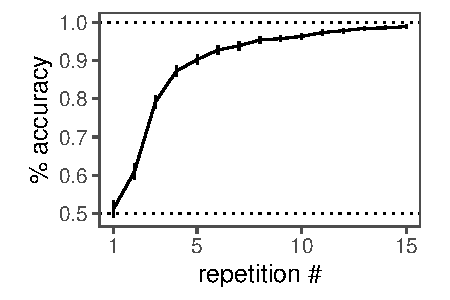
\includegraphics[scale=.8]{sec1-convergence.pdf}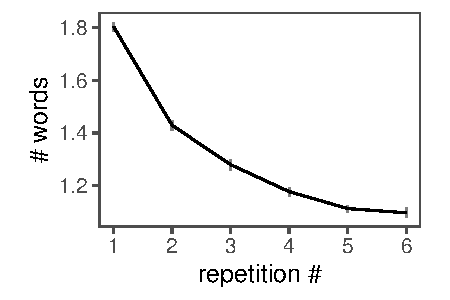
\includegraphics[scale=.8]{sec1-efficiency}
  \caption{\emph{Pairs of agents learn to successfully coordinate on efficient ad hoc conventions over repeated interactions.} (A) agents converge on accurate communication systems in Simulation 1.1, where only single-word utterances are available, and (B) converge on shorter, more efficient conventions in Simulation 1.2, where multi-word utterances were available. Error bars are bootstrapped 95\% CIs across 1000 trajectories, computed within each repetition block of two trials.}
  \label{fig:sec1model}
\end{figure}

\subsection{Simulation 1.1: Pure coordination}


We build up to our explanation of increasing efficiency by first exploring a traditional signaling game scenario with only one-word utterances.
This simulation tests the most fundamental competency for any model of \emph{ad hoc} coordination: agents are able to coordinate on a communication system in the absence of shared priors. 
We consider the simplest possible reference game with two objects, $\mathcal{O} = \{\orangecircle, \bluesquare\}$, where the speaker must choose between two one-word utterances $\mathcal{U} = \{u_1, u_2\}$ with equal production cost. 

We walk explicitly through the first step of the simulation to illustrate the model's dynamics (see Fig.~\ref{fig:path-dependence}).
Suppose the target object presented to the speaker agent on the initial trial is $\orangecircle$.
Both utterances are equally likely to apply to either object under the uniform lexical prior, hence each utterance is expected to be equally (un)informative. 
The speaker's utility therefore reduces to sampling an utterance at random $u~\sim~S(u\,|\, \orangecircle)$.
Suppose $u_1$ is sampled.
The listener then hears this utterance and selects an object according to their own expected utility under their uniform lexical prior, which also reduces to sampling an object at random $o \sim L(o | u_1)$.
Suppose they choose, $ \orangecircle$, a correct response.
Both agents may use the resulting tuple $D = \{ \orangecircle^*, u_1,  \orangecircle\}$, depicted in the top row in Fig.~\ref{fig:path-dependence} to update their beliefs about the lexicon their partner is using.
\begin{align}
P_S(\phi | D) & \propto L_0( \orangecircle\, |\, u_1, \phi)P(\phi)\nonumber \\
P_L(\phi | D) & \propto S_1(u_1 \,|\, \orangecircle^*, \phi)P(\phi)\nonumber
\end{align}
They then proceed to the next trial, where they use this updated posterior distribution to produce or interpret language instead of their prior.
To examine how the dynamics of this updating process unfold over further rounds, we simulated 1000 such trajectories.
The trial sequence was structured as a repeated reference game, containing 30 trials structured into 15 repetition blocks.
The two objects appeared in a random order within each block, and agents swapped roles at the beginning of each block.
We show representative behavior at soft-max optimality parameter values $\alpha_L = \alpha_S = 8$ and memory discounting parameter $\beta = 0.8$, but find similar behavior in a wide regime of parameter values (see Appendix Fig.~\ref{fig:arbitrariness_grid}).



We highlight several key results from this simulation.
First, and most fundamentally, the communicative success of the dyad rises over the course of interaction: the listener is able to more accurately select the intended target object (see Fig.~\ref{fig:sec1model}A). 
Second, the initial symmetry between meanings in the prior is broken by initial choices, leading to \emph{arbitrary} but \emph{stable} mappings in future rounds.
Because agents were initialized with the same priors in every trajectory, trajectories only diverged when different actions happen to be sampled.
This can be seen by examining the path-dependence of subsequent beliefs based on the outcome of the initial trial in Fig.~\ref{fig:path-dependence}.
Third, we observe the influence of mutual exclusivity via Gricean pragmatic reasoning: agents also make inferences about objects and utterances that were \emph{not} chosen. 
For example, observing $D = \{(\orangecircle^*, u_2, \orangecircle)\}$ provides evidence that $u_1$ likely does not mean $\orangecircle$ (e.g.~the third row of Fig.~\ref{fig:path-dependence}, where hearing $u_2$ refer to $\orangecircle$ immediately led to the inference that $u_1$ likely refers to $\bluesquare$).

\subsection{Simulation 1.2: Increasing efficiency}

Next, we show how our model explains speakers' gains in efficiency over multiple interactions. 
For efficiency to change at all, speakers must be able to produce utterances that vary in length. 
For this simulation, we therefore extend the model to allow for multi-word utterances by allowing speakers to combine together multiple primitive utterances.
Intuitively, human speakers form longer initial description by combining a collection of simpler descriptions (e.g. ``kind of an X, or maybe a Y with Z on top''). 
This raises a problem about how the meaning of a multi-word utterance $\mathcal{L}_\phi(u_1u_2)$ is derived from its components $\mathcal{L}_\phi(u_1)$ and $\mathcal{L}_\phi(u_2)$.
To capture the basic desideratum that an object should be more likely to be chosen by $L_0$ when more components of the longer utterance apply to it, we adopt a standard conjunctive semantics:
$$\mathcal{L}_\phi(u_iu_j, o) = \mathcal{L}_\phi(u_i, o) \times \mathcal{L}_\phi(u_j, o)$$
One subtle consequence of a conjunctive Boolean semantics is the possibility of contradictions. 
For example, under a possible lexicon where $\phi(u_1)=\bluesquare$ and $\phi(u_2)=\orangecircle$, the multi-word utterance $u_1u_2$ is not only false of the particular referents in the current context, it is false of all \emph{possible} referents, reflecting a so-called truth-gap \cite{Strawson50_OnReferring,van1966singular}. 
We assume such an utterance is uninterpretable and simply disregarded without changing the literal listener $L_0$'s beliefs. 
While this assumption is sufficient for our simulations, we regard this additional complexity as a limitation of classical truth-conditional semantics  \cite{degen2020redundancy} and show in Appendix B that switching to a continuous semantics with lexical values in the interval $[0,1]$ may better capture the notion of redundancy that motivates speakers to initially produce longer utterances.

Now, we consider a scenario with the same two objects as in Simulation 1.1, but give the speaker four primitive utterances $\{u_1, u_2, u_3, u_4\}$ instead of only two, and allow two-word utterances such as $u_1u_2$.
We established in the previous section that successful \emph{ad hoc} conventions can emerge even in a state of pure uncertainty, but human participants in repeated reference games typically bring some prior expectations about language into the interaction.
For example, a participant who hears `ice skater' on the first round of the task in \citeA{ClarkWilkesGibbs86_ReferringCollaborative} may be more likely to select some objects more than others while still having substantial uncertainty about the intended target (e.g. over three of the twelve tangram that have some resemblance to an ice skater).
%This observation is key to understanding why speakers may initially use longer utterances in repeated reference games with ambiguous stimuli. 
%Under a uniform prior, where all words are expected to be equally meaningless to one's partner, longer utterances would have no additional value. 
%Under a concentrated prior, where there already exists a strong convention for a short label, that label would suffice and a longer utterance would be completely redundant.
We thus initialize both agents with weak biases $\delta$ (represented in compressed matrix form in Fig.~\ref{fig:sec1efficiency}):
\begin{align}
\phi(u_1), \phi(u_2) \sim \textrm{Categorical}(0.5 + \delta) \nonumber\\
\phi(u_3), \phi(u_4) \sim \textrm{Categorical}(0.5 - \delta) \nonumber
\end{align}

\begin{figure}[t]
\centering
    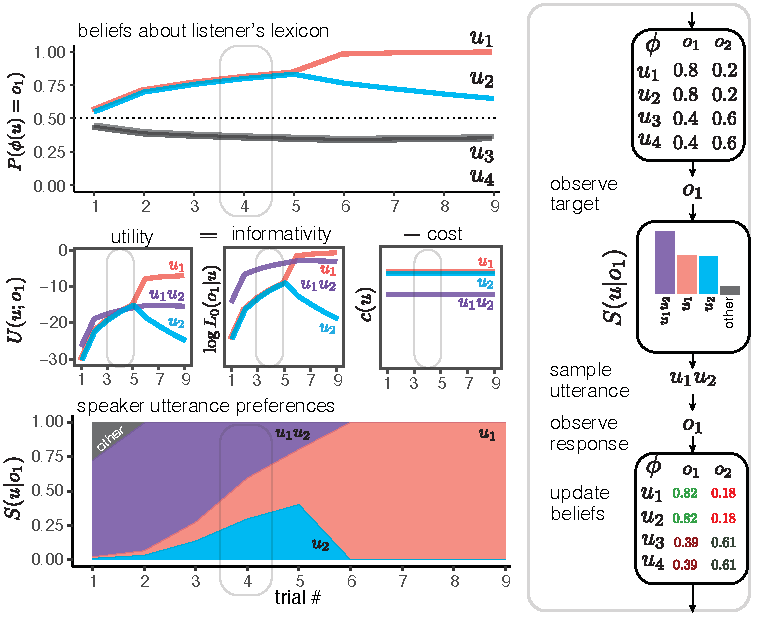
\includegraphics[scale=.9]{sec1-reduction_example}
  \caption{\emph{Schematic of speaker for first trial of Simulation 1.2.} The speaker begins with uncertainty about the meanings in the listener's lexicon (e.g. assigning 55\% probability to the possibility that utterance $u_1$ means object $o_1$.) A target $o_1$ is presented, and the speaker samples an utterance from the distribution $S(u|o_1)$. Finally, they observe the listener's response and update their beliefs. Due to the compositional semantics of the utterance $u_1u_2$, the speaker becomes increasingly confident that both component primitives, $u_1$ and $u_2$, apply to object $o_1$ in their partner's lexicon.}
  \label{fig:sec1efficiency}
\end{figure}


\begin{figure*}[t]
\centering
    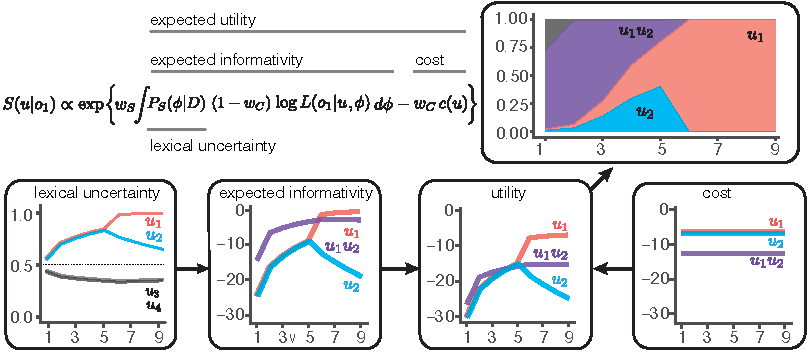
\includegraphics[scale=1]{sec1-reduction_schematic}
  \caption{\emph{Internal state of speaker in example trajectory from Simulation 1.2.} Each term of the speaker's utility (Eq. \ref{eq:marginalized}) is shown throughout an interaction. When the speaker is initially uncertain about meanings (far left), the longer utterance $u_1u_2$ has higher expected informativity (center-left) and therefore higher utility (center-right) than the shorter utterances $u_1$ and $u_2$, despite its higher cost (far-right). As the speaker observes several successful interactions, they update their beliefs and become more confident about the meanings of the component lexical items $u_1$ and $u_2$. As a result, more efficient single-word utterances gradually gain in utility as cost begins to dominate the utility. On trial 5, $u_1$ is sampled, breaking the symmetry between utterances.}
  \label{fig:sec1internals}
\end{figure*}

As in Simulation 1.1, we simulated 1000 distinct trajectories of dyadic interaction between agents.
Utterance cost was defined to be the number of `words' in an utterance, so $c(u_1) =1$ and $c(u_1u_2)=2$.
As shown in Fig.~\ref{fig:sec1model}B, our speaker agent initially prefers longer utterance (mean length $\approx 1.5$ on first block) but rapidly converges to shorter utterances after several repetitions (mean length $\approx 1$ on final block), qualitatively matching the curves measured in the empirical literature.

To illustrate in detail how our model derives this behavior, we walk step-by-step through a single trial (Fig. \ref{fig:sec1efficiency}).
Consider a speaker who wants to refer to object $\bluesquare$. 
They expect their partner to be slightly more likely to interpret their language using a lexicon in which $u_{1}$ and $u_{2}$ apply to this object, due to their weak initial biases. 
However, there is still a reasonable chance ($p=0.45$) that either $u_1$ or $u_2$ alone will be interpreted to mean $\orangecircle$, giving their partner false beliefs. 
To see why our speaker model initially prefers the longer utterance $u_{1}u_{2}$ to hedge against this possibility, despite its higher production cost, consider the expected informativity of $u_1u_2$ under different possible lexicons.
The possibility with highest probability is that both $\phi(u_1) = \phi(u_2) = \bluesquare$ in the listener's lexicon ($p = 0.55^2 \approx 0.3$), in which case the listener will correctly identify $\bluesquare$ with high probability.
The possibility that both $\phi(u_1)=\phi(u_2) = \orangecircle$ in the listener's lexicon is only $p=0.45^2 \approx 0.2$, in which case the listener will erroneously select $\orangecircle$.
In the mixed cases, where $\phi(u_1) = \orangecircle, \phi(u_2) = \bluesquare$ or $\phi(u_1) = \bluesquare, \phi(u_2) = \orangecircle$ in the listener's lexicon ($p = 2 \cdot 0.45 * 0.55 \approx 0.5$), the utterance would be a interpreted as a contradiction and the listener would not change their prior beliefs.
Because the speaker's informativity is defined using the log probability of the listener's belief, the utility of giving the listener a false belief, $\log(\epsilon)$ is significantly worse than simply being uninformative, i.e. $\log(0.5)$, and the longer utterance minimizes this harm.

Following the production of a conjunction, the speaker observes the listener's response (say, $\bluesquare$).
This allows both agents to become more confident that the component utterances $u_1$ and $u_2$ mean $\bluesquare$ in their updated posterior over the listener's lexicon.
This credit assignment to individual lexical items is a consequence of the compositional meaning of longer utterances in our simple grammar.
The listener knows a speaker for whom either $u_1$ or $u_2$ individually means $\bluesquare$ would have been more likely to say $u_1u_2$ than a speaker for whom either component meant $\orangecircle$; and similarly for the speaker reasoning about possible listeners.
Consequently, the probability of both mappings increases.

Fig.~\ref{fig:sec1internals} shows the trajectories of internal components of the speaker utility as the interaction continues.
We assume for illustrative purposes in this example that $\bluesquare$ continues to be the target on each trial and the same agent continues to be the speaker.
As the posterior probability that individual primitive utterances $u_1$ and $u_2$ independently mean $\bluesquare$ increases (far left), the marginal gap in informativity between the conjunction and the shorter components gradually decreases (center left).
As a consequence, production cost increasingly dominates the utility (center-right). 
After several trials of observing a successful listener response given the conjunction, the \emph{informativity} of the two shorter utterances reaches parity with the conjunction but the cost makes the shorter utterances more attractive (yielding a situation now similar to the outset of Simulation 1.1).
Once the speaker samples one of the shorter utterances (e.g. $u_1$), the symmetry collapses and that utterance remains most probable in future rounds, allowing for a stable and efficient \emph{ad hoc} convention.
Thus, increasing efficiency is derived as a rational consequence of uncertainty and partner-specific inference about the listener's lexicon.
For these simulations, we used $\alpha_S = \alpha_L = 8, w_c = 0.24, \beta=0.8$ but the qualitative reduction effect is found over a range of different parameters (see Appendix Fig. \ref{fig:conjunction_grid}). 

%\paragraph{Model comparison}
%
%Here we compare this model to several simpler baselines to establish which components of the model are necessary and sufficient for the desired behavior.
%
%\rdh{e.g., no pragmatics, pragmatics only in learning rule or only in decision rule instead of both, simpler pragmatics (reasoning about $L_0$ instead of $L_1$), point estimate instead of uncertainty, effect of different parameter regimes.} 
%
%\rdh{It may also be useful to explicitly show that the simpler Roth-Erev RL updating from this literature doesn't reduce, or even better show that this kind of simpler update rule is equivalent to something within our framework as a point estimate representation with maximum likelihood or something...?}

%In the limit, it doesn't matter whether you have pragmatics in both learning rule or decision rule. 
%In case where it's only in production rule, you'll produce the data with the necessary biases in learning.

\subsection{Discussion}

The simulations presented in this section aimed to establish a rational explanation for feedback-sensitive increases in efficiency over the course of \emph{ad hoc} convention formation.
Speakers initially hedge their descriptions under uncertainty about the lexical meanings their partner is using, but are able to get away with less costly components of those descriptions as their uncertainty decreases.
This explanation recalls classic observations about \emph{hedges} (expressions like \emph{sort of} or morphemes like \emph{-ish}) that explicitly mark provisionality, such as \emph{a sort of silvery purple colored car} \cite{lakoff1975hedges,Fraser10_Hedging,MedlockBriscoe07_HedgeClassification}.
\citeA{BrennanClark96_ConceptualPactsConversation} counted hedges across repetitions of a repeated reference game, finding a greater occurrence of hedges on early trials than later trials and a greater occurrence under more ambiguous contexts.
While our model does not include hedges, it is possible to understand this behavior as an explicit or implicit marker of the lexical uncertainty construct in our account.
Our account is also broadly consistent with recent analyses of exactly \emph{what} gets reduced in a large corpus of repeated reference games \cite{hawkins2020characterizing}.
These analyses found that entire modifying clauses are more likely to be dropped at once than would be expected by random and independent corruption.
In other words, speakers apparently begin by combining multiple descriptive modifiers and collapse to retain only one of these `units' contingent on evidence that their partner understands.

Why has this phenomenon remained outside the explanatory scope of previous models?
Our account differs in both level of analysis and model complexity.
For example, the influential \emph{interactive alignment} account proposes that that speakers adapt and coordinate on meaning through priming mechanisms that allow phonetic or syntactic features associated with lexical items to percolate up to strengthen higher levels of representation \cite{pickering2004toward, pickering2006alignment,roelofs1992spreading}.
While priming mechanisms are certainly at play in repeated reference tasks, especially when listeners engage in extensive dialogue and alternate roles, it is not clear why priming alone would lead descriptions to get shorter as opposed to aligning on the same longer initial description.
Furthermore, priming cannot explain why speakers still converge to more efficient labels even when the listener is prevented from saying anything at all and only sparse, non-verbal feedback is provided; conversely, speakers continue using longer descriptions when they receive non-verbal feedback that the listener is repeatedly making errors (\citeNP{KraussWeinheimer66_Tangrams}; see also \citeNP{hawkins2020characterizing}).
In these cases, there are no linguistic features available for priming or alignment to act upon.
Our computational-level account is not mutually exclusive with these process-level principles and does not in any way falsify or undermine them.
Explaining when and why speakers believe that shorter descriptions suffice requires additional computational-level principles to be considered, which we hope will lead to further enrichment of algorithms at the process level.

Another prominent account proposes that speakers coordinate on meaning using some lexical update rule that makes utterances more likely to be produced after communicative successes and less likely after communicative failures.
This account has often been implemented using a simple variant of reinforcement learning (RL) such as Roth-Erev learning \cite{erev1998predicting,steels_self-organizing_1995,barr_establishing_2004,young_evolution_2015}.
While such minimal rules allow groups to reach consensus, it is challenging to explain the full suite of phenomena we have explored in this section.
First, for most of these models, it is not clear how simply reinforcing initially long descriptions could lead utterances to get shorter. 
Second, in the rare cases that have allowed longer utterances to be constructed compositionally from more primitive utterances, reduction has been hard-coded as a kind of $\epsilon$-greedy exploration where the speaker has a fixed probability of dropping a random token at each point in time \cite{beuls2013agent,steels2016agent}.
Such random dropping, however, is inconsistent with early control experiments by \citeA{HupetChantraine92_CollaborationOrRepitition} where participants were asked to repeatedly refer to the same targets for a \emph{hypothetical} partner to see later, such that any effects of familiarity or repetition on the part of the speaker would be the same as the interactive task \cite<see also>{GarrodFayLeeOberlanderMacLeod07_GraphicalSymbolSystems}. 
No evidence of reduction was found in this case, and in some cases utterances actually grew longer.
Third, even if this problem were fixed by extending the update rule to be contingent on interaction, it is not clear why a speaker would initially prefer to produce longer utterances over shorter utterances.
%Whatever drives increasing efficiency cannot be explained through speaker laziness, it must be a result of contingent \emph{interaction} between partners.
%Second, it is inconsistent with the multi-partner settings explored by \citeA{wilkes-gibbs_coordinating_1992}, which we explore further in \textbf{P2}: It is not clear why a speaker who shortened their descriptions due to an $\epsilon$-greedy process would suddenly switch back to longer utterances when their partner is exchanged.

Importantly, these limitations do not stem from the RL framework itself, but from the simplifying assumption that the probability of taking actions should be directly tied to the previous outcomes of those actions.
CHAI preserves a core idea from these accounts --- the ability to dynamically adapt one's behavior contingent on one's partner's --- but disentangles the inference problem (i.e. estimating a partner's underlying lexicon) from the decision problem (i.e. deciding which action to take with these estimates in hand).
Introducing the latent variable of the lexicon as an intermediate construct allows the model to be more explanatory while also necessarily increasing its complexity.
Importantly, more sophisticated \emph{model-based} reinforcement learning algorithms make a similar distinction and may consequently be flexible enough to account for this phenomenon (see \citeNP{gershman2015novelty} for an explicit connection between hierarchical Bayes and an RL algorithm known as TD-learning; but see \citeNP{velez2021learning} for outstanding problems associated with bridging these perspectives).
%For instance, hierarchical architectures that appropriately incorporate compositionality or incrementality into the speaker's production model may be able to reinforce component parts of longer utterances in the shared history \cite<e.g.>{hawkins2019continual}.
%Still, such an approach would have more in common with our proposal than to the model-free heuristics in the existing literature.

Finally, while our simulations captured several core features of the reduction phenomenon, they have only scratched the surface of its empirical complexity.
First, our simulations only consider two-word descriptions with homogenous uncertainty over the components, while the semantic components of real initial descriptions have more heterogeneity. 
It remains an open question as to how best to instantiate more realistic priors in our model that can predict more fine-grained patterns. 
For example, early hand-tagged analyses by \citeA{Carroll80_NamingHedges} found that in three-quarters of transcripts from \citeA{krauss_changes_1964} the conventions that participants eventually converged upon were prominent in some syntactic construction at the beginning, often as a head noun that was initially modified or qualified by other information. 
Second, gains in efficiency associated with \emph{ad hoc} conventions do not necessarily translate into shorter utterances.
Outside of the domain of reference games, speakers often have control over what they want to convey and may use the efficiency afforded by their new conventions to express more information in the same number of words rather than the same amount of information in fewer words \cite{effenberger2021analysis}. 
Once a convention is formed, it can be used as a new primitive to bootstrap further conventions and convey ever-more-sophisticated meanings \cite{mccarthy2021learning}.





